% В этом документе преамбула

\documentclass[a4paper,12pt]{article}

\usepackage{lscape} % горизонтальный режим
\usepackage{pdflscape}

\usepackage{lipsum} % тестовые тексты

%%% Работа с русским языком
\usepackage{cmap}					% поиск в PDF
\usepackage{mathtext} 				% русские буквы в формулах
\usepackage[T2A]{fontenc}			% кодировка
\usepackage[utf8]{inputenc}			% кодировка исходного текста
\usepackage[english,russian]{babel}	% локализация и переносы
\usepackage{indentfirst}			% чтобы первый абзац в разделе отбивался красной строкой
\frenchspacing						% тонкая настройка пробелов
\usepackage{gensymb}				% символы по типу градусов
\usepackage{algorithm}				% для алгоритмов
\usepackage{algorithmic}			% для алгоритмов

%%% Приведение начертания букв и знаков к русской типографской традиции
\renewcommand{\epsilon}{\ensuremath{\varepsilon}}
\renewcommand{\phi}{\ensuremath{\varphi}}			% буквы "эпсилон"
\renewcommand{\kappa}{\ensuremath{\varkappa}}		% буквы "каппа"
\renewcommand{\le}{\ensuremath{\leqslant}}			% знак меньше или равно
\renewcommand{\leq}{\ensuremath{\leqslant}}			% знак меньше или равно
\renewcommand{\ge}{\ensuremath{\geqslant}}			% знак больше или равно
\renewcommand{\geq}{\ensuremath{\geqslant}}			% знак больше или равно
\renewcommand{\emptyset}{\varnothing}				% знак пустого множества

%%% Дополнительная работа с математикой
\usepackage{amsmath,amsfonts,amssymb,amsthm,mathtools,esint} % AMS
\usepackage{wasysym}
\usepackage{icomma} % "Умная" запятая: $0,2$ --- число, $0, 2$ --- перечисление

%% Номера формул
\mathtoolsset{showonlyrefs=true} % Показывать номера только у тех формул, на которые есть \eqref{} в тексте.

%% Свои команды

% операции, не определённые (или имеющие иные обохначения) в мат. пакетах
\DeclareMathOperator{\sgn}{\mathop{sgn}}				% ф-ия sgn
\renewcommand{\tg}{\mathop{\mathrm{tg}}\nolimits}		% обозначение тангенса

%% Перенос знаков в формулах (по Львовскому)
\newcommand*{\hm}[1]{#1\nobreak\discretionary{}
{\hbox{$\mathsurround=0pt #1$}}{}}

%%% Работа с картинками
\usepackage{graphicx}  				% Для вставки рисунков
\graphicspath{{images/}{images2/}}  % папки с картинками
\setlength\fboxsep{3pt} 			% Отступ рамки \fbox{} от рисунка
\setlength\fboxrule{1pt} 			% Толщина линий рамки \fbox{}
\usepackage{wrapfig} 				% Обтекание рисунков текстом

%%% Работа с таблицами
\usepackage{array,tabularx,tabulary,booktabs} 	% Дополнительная работа с таблицами
\usepackage{longtable}  						% Длинные таблицы
\usepackage{multirow}							% Слияние строк в таблице

%%% Теоремы

\newtheoremstyle{break}% name
	{}%         Space above, empty = `usual value'
	{}%         Space below
	{\itshape}% Body font
	{}%         Indent amount (empty = no indent, \parindent = para indent)
	{\bfseries}% Thm head font
	{.}%        Punctuation after thm head
	{\newline}% Space after thm head: \newline = linebreak
	{}%         Thm head spec
\theoremstyle{break}

% \theoremstyle{plain} % Стиль по умолчанию
\newtheorem{theorem}{Теорема}[section]
\newtheorem{lemma}{Лемма}[section]
\newtheorem{definition}[theorem]{Определение}
\newtheorem{property}{Свойство}
 
\newtheorem{corollary}{Следствие}[theorem]

\newtheoremstyle{example}	% style name
	{2ex}					% above space
	{2ex}					% below space
	{}						% body font
	{}						% indent amount
	{\bf}				% head font
	{.}						% post head punctuation
	{\newline}				% post head punctuation
	{\thmname{#1}\thmnumber{ #2}\thmnote{ (#3)}}						% head spec

\theoremstyle{example}
\newtheorem{exmp}{Пример}[section]
 
\theoremstyle{remark} % "Примечание"
\newtheorem*{nonum}{Решение}
\newtheorem*{evidence}{Доказательство}
\newtheorem*{remark}{Примечание}

%%% Программирование
\usepackage{etoolbox} % логические операторы

%%% Страница
\usepackage{extsizes} % Возможность сделать 14-й шрифт
\usepackage{geometry} % Простой способ задавать поля
	\geometry{top=15mm}
	\geometry{bottom=35mm}
	\geometry{left=10mm}
	\geometry{right=10mm}

%\usepackage{fancyhdr} % Колонтитулы
% 	\pagestyle{fancy}
 	%\renewcommand{\headrulewidth}{0pt}  % Толщина линейки, отчеркивающей верхний колонтитул
% 	\lfoot{Нижний левый}
% 	\rfoot{Нижний правый}
% 	\rhead{Верхний правый}
% 	\chead{Верхний в центре}
% 	\lhead{Верхний левый}
%	\cfoot{Нижний в центре} % По умолчанию здесь номер страницы

\usepackage{setspace} % Интерлиньяж (межстрочные интервалы)
%\onehalfspacing % Интерлиньяж 1.5
%\doublespacing % Интерлиньяж 2
%\singlespacing % Интерлиньяж 1

\usepackage{lastpage} % Узнать, сколько всего страниц в документе.

\usepackage{soulutf8} % Модификаторы начертания

\usepackage{hyperref}
\usepackage[usenames,dvipsnames,svgnames,table,rgb]{xcolor}
\hypersetup{				% Гиперссылки
    unicode=true,           % русские буквы в раздела PDF
    pdftitle={Заголовок},   % Заголовок
    pdfauthor={Автор},      % Автор
    pdfsubject={Тема},      % Тема
    pdfcreator={Создатель}, % Создатель
    pdfproducer={Производитель}, % Производитель
    pdfkeywords={keyword1} {key2} {key3}, % Ключевые слова
    colorlinks=true,       	% false: ссылки в рамках; true: цветные ссылки
    linkcolor=MidnightBlue, % внутренние ссылки
    citecolor=black,        % на библиографию
    filecolor=magenta,      % на файлы
    urlcolor=blue           % на URL
}

\usepackage{csquotes} % Еще инструменты для ссылок

%\usepackage[style=authoryear,maxcitenames=2,backend=biber,sorting=nty]{biblatex}

\usepackage{multicol} % Несколько колонок

%%% Работа с графикой
\usepackage{tikz}
\usetikzlibrary{calc}
\usepackage{tkz-euclide}
\usetikzlibrary{arrows}
\usepackage{pgfplots}
\usepackage{pgfplotstable}

%%% Настройка подписей к плавающим объектам
% \usepackage{floatrow}	% размещение
\usepackage{caption}	% начертание
\captionsetup[figure]{labelfont=bf,textfont=it,font=footnotesize}	% нумерация и надпись курсивом
% для подфигур: заголовок подписи полужирный, текст заголовка обычный
% выравнивание является неровным (т.е. выровненным по левому краю)
% singlelinecheck = off означает, что настройка выравнивания используется, даже если заголовок имеет длину только одну строку.
% если singlelinecheck = on, то заголовок всегда центрируется, когда заголовок состоит только из одной строки.
\captionsetup[subfigure]{labelfont=bf,textfont=normalfont,singlelinecheck=off,justification=raggedright}

%%% Stuff для листинга
\usepackage{listings}
\usepackage{xcolor}

\colorlet{mygray}{black!30}
\colorlet{mygreen}{green!60!blue}
\colorlet{mymauve}{red!60!blue}

\lstset{
	backgroundcolor=\color{gray!10},  
	basicstyle=\ttfamily,
	columns=fullflexible,
	breakatwhitespace=false,      
	breaklines=true,                
	captionpos=b,                    
	commentstyle=\color{mygreen}, 
	extendedchars=true,              
	frame=single,                   
	keepspaces=true,             
	keywordstyle=\color{blue},      
	language=c++,                 
	numbers=none,                
	numbersep=5pt,                   
	numberstyle=\tiny\color{blue}, 
	rulecolor=\color{mygray},        
	showspaces=false,               
	showtabs=false,                 
	stepnumber=5,                  
	stringstyle=\color{mymauve},    
	tabsize=3,                      
	title=\lstname                
}

% для извращённых начертаний
\usepackage{mathrsfs}

\usepackage{makecell}
\setcellgapes{3pt}

% Зачёркивание символов
\usepackage{cancel}

% перечисления с буквами
\usepackage{enumitem}

\title{Теория вероятностей и мат. статистика}
\date{27.03.2020}
\author{Почаев Никита Алексеевич, гр. 8381 \\ \href{mailto:pochaev.nik@gmail.com}{pochaev.nik@gmail.com} \\ Преподаватель: Малов Сергей Васильевич}

\begin{document}
	
\renewcommand{\figurename}{Рисунок}

\maketitle

\section*{Случайные величины}

Случайная величина $\xi: \Omega \to \mathbb{R}$ измеримая функция.
\[ (\Omega, \mathcal{F}, P) \mapsto (\mathbb{R}, \mathscr{D}_1, \mathscr{P}_{\xi}) \]
\noindent $\mathscr{P}_{\xi}$ - распределение, $\mathscr{P}_{\xi}(I) = P(\omega: \xi(\omega) \in I)$

\noindent Функция распределения: $F_{\xi}(x) = P(\omega: \xi(\omega) < x)$

\subsection*{Задача 1.}

Найти функцию распределения числа очков, выпадающих на кубике.

\noindent \textit{Решение:}

$F\xi(x)$ - вероятность, что выпало $<x$ очков.

\[
F_{\xi} (x) = 
\begin{cases}
	0, &x \le 1 \text{\textcolor{Grey}{ (<0 очков не бывает)}} \\
	\frac{1}{6}, &x \in (1, 2] \text{\textcolor{Grey}{ (выпадает $\le$ 1)}} \\
	\frac{1}{3}, &x \in (2, 3] \text{\textcolor{Grey}{ (выпадает $\le$ 2)}} \\
	\frac{1}{2}, &x \in (3, 4] \\
	\frac{2}{3}, &x \in (4, 5] \\
	\frac{5}{6}, &x \in (5, 6] \\
	1, &x > 6 \text{\textcolor{Grey}{ (обязательно выпадет очков $\le$ 6)}}
\end{cases}
\]

\begin{figure}[H]
	\center{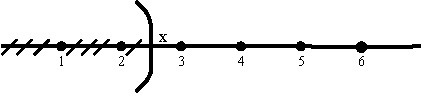
\includegraphics[scale=0.9]{./media/Homework-27-03-20_1.pdf}}
\end{figure}
\begin{figure}[H]
	\center{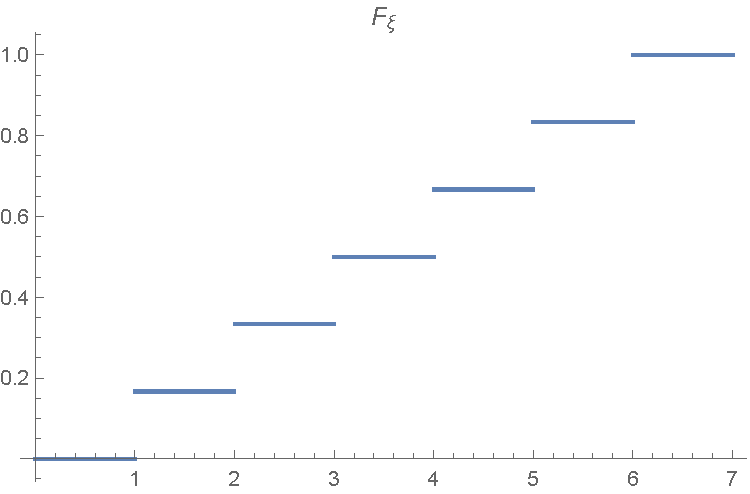
\includegraphics[scale=0.9]{./media/Homework-27-03-20_2.pdf}}
\end{figure}

\subsection*{Задача 2.}

Найти функцию распределения решек, выпавших до 1-ого орла при бросании монеты.

\noindent \textit{Решение:}

$\xi$ - искомая величина (число решек до 1-ого орла), переформулируя,  $\xi$ - число успехов (выпадение решки) до 1-ой неудачи (выпадение орла).

Вероятность выпадения решки: $P(\text{'Р'}) = \frac{1}{2}$.

По формуле испытания Бернулли: $p(\xi = k) = p^k(1-p) = \frac{1}{2} \cdot \frac{1}{2^k} = \frac{1}{2^{k+1}}$.
\begin{figure}[H]
	\center{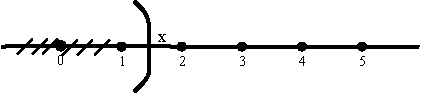
\includegraphics[scale=0.9]{./media/Homework-27-03-20_3.pdf}}
\end{figure}
\[ F_{\xi}(x) = \sum_{k < x} P(\xi = k) = \underbrace{\sum_{k=0}^{k<x} \frac{1}{2^{k+1}}}_{\frac{1}{2} + \frac{1}{4} + \frac{1}{8} + \dots} =
\begin{cases}
	0, x \le 0 \\
	1 - \frac{1}{2^{k+1}}, x \in (k, k+1], k = 0,1,\dots
\end{cases}
\]
где $\sum_{k < x} P(\xi = k)$ - все случаи, когда выпало $<x$.
\begin{figure}[H]
	\center{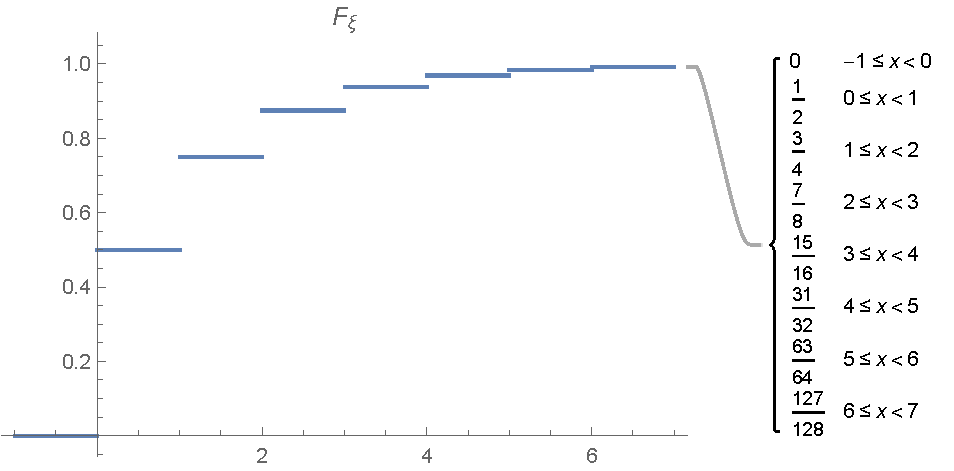
\includegraphics[scale=0.9]{./media/Homework-27-03-20_4.pdf}}
\end{figure}

\subsection*{Задача 3.}

Точка бросается наугад в интервале $[0,1], \xi$ - координаты точки.
\[ F_{\xi}(x) =
\begin{cases}
	0, x \le 0 \\
	x, x \in (0,1] \\
	1, x > 1 \text{\textcolor{Grey}{ (обязательно будет $\le$ 1)}}
\end{cases}
\]
\[ P(\xi < x) = P(\xi \in[0,1]) \]
\begin{figure}[H]
	\center{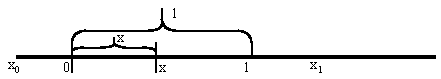
\includegraphics[scale=1]{./media/Homework-27-03-20_5.pdf}}
\end{figure}
Вероятность отрезка $[0,x) = \frac{x}{1} = x$.
\begin{figure}[H]
	\center{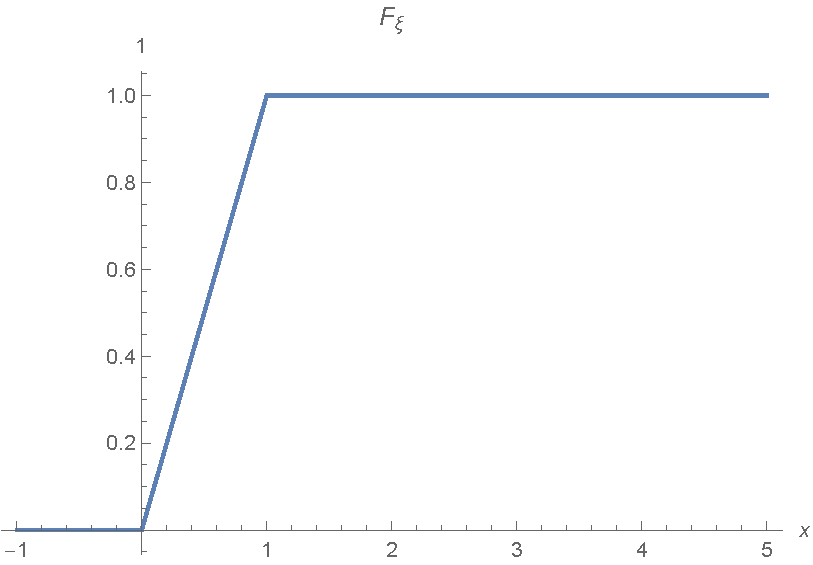
\includegraphics[scale=0.85]{./media/Homework-27-03-20_6.pdf}}
\end{figure}
\[ P(\xi < x) = P(\xi \in [0,x)) \]

\subsection*{Задача 4.}

Бросается два игральных кубика, дискретная случайная величина $\xi$ - сумма очков. Найти $F_{\xi} = ?$

\noindent \textit{Решение:}

Рассмотрим все возможные варианты выпадения очков на обоих кубиках и их суммы:
\begin{table}[H]
	\centering
	\begin{tabular}{|c|c|c|c|c|c|c|c|c|c|c|c|}
		\hline
		$\xi$ & 2     & 3                                                        & 4                                                                      & 5                                                                              & 6                                                                                         & 7                                                                                                    & 8                                                                                         & 9                                                                              & 10                                                                  & 11                                                       & 12    \\ \hline
		& (1;1) & \begin{tabular}[c]{@{}c@{}}(1;2)\\ \\ (2;1)\end{tabular} & \begin{tabular}[c]{@{}c@{}}(1;3)\\ \\ (2;2)\\ \\ (3,1)\end{tabular} & \begin{tabular}[c]{@{}c@{}}(1;4)\\ \\ (2;3)\\ \\ (3;2)\\ \\ (4;1)\end{tabular} & \begin{tabular}[c]{@{}c@{}}(1;5)\\ \\ (2;4)\\ \\ (3;3)\\ \\ (4;2)\\ \\ (5;1)\end{tabular} & \begin{tabular}[c]{@{}c@{}}(1;6)\\ \\ (2;5)\\ \\ (3;4)\\ \\ (4;3)\\ \\ (5;2)\\ \\ (6;1)\end{tabular} & \begin{tabular}[c]{@{}c@{}}(2;6)\\ \\ (3;5)\\ \\ (4;4)\\ \\ (5;3)\\ \\ (6;2)\end{tabular} & \begin{tabular}[c]{@{}c@{}}(3;6)\\ \\ (4;5)\\ \\ (5;4)\\ \\ (6;3)\end{tabular} & \begin{tabular}[c]{@{}c@{}}(4;6)\\ \\ (5;5)\\ \\ (6;4)\end{tabular} & \begin{tabular}[c]{@{}c@{}}(5;6)\\ \\ (6;5)\end{tabular} & (6;6) \\ \hline
	\end{tabular}
\end{table}
Так как каждый кубик подбрасывается независимо от другого, то согласно принципу произведения, общее число вариантов выпадения двух цифр на кубиках равно:
\[ \# \Omega = 6 \cdot 6 = 36 \]
Событие $A_{\xi}$ - выпало суммарно $\xi$ очков, тогда количество исходов для каждой суммы очков будет равно:
\begin{table}[H]
	\centering
	\begin{tabular}{|c|c|c|c|c|c|c|c|c|c|c|c|}
		\hline
		$\xi$        & 2 & 3 & 4 & 5 & 6 & 7 & 8 & 9 & 10 & 11 & 12 \\ \hline
		$\# A_{\xi}$ & 1 & 2 & 3 & 4 & 5 & 6 & 5 & 4 & 3  & 2  & 1  \\ \hline
	\end{tabular}
\end{table}
\noindent Таким образом,
\[ x \le 2 \Rightarrow F_{\xi} = P(\xi < x) = \frac{0}{36} = 0 \]
\[ x \in (2,3] \Rightarrow F_{\xi} = P(\xi < x) = \frac{\#A_1}{\#\Omega} = \frac{1}{36} \]
\[ x \in (3,4] \Rightarrow F_{\xi} = P(\xi < x) = \frac{\#A_1 + \#A_2}{\#\Omega} = \frac{1+2}{36} = \frac{1}{12} \]
\[ x \in (4,5] \Rightarrow F_{\xi} = \frac{1 + 2 + 3}{36} = \frac{6}{36} = \frac{1}{6} \]
\[ \dots \]
В результате получаем функцию распределения:
\[
F_{\xi}(x) = 
\begin{cases}
	0, x \le 2 \\
	\frac{1}{36}, &x \in (2,3] \\
	\frac{1}{12}, &x \in (3,4] \\
	\frac{1}{6}, &x \in (4,5] \\
	\frac{10}{36} = \frac{5}{18}, &x \in (5,6] \\
	\frac{15}{36}=\frac{5}{12}, &x \in (6,7] \\
	\frac{21}{36}=\frac{7}{12}, &x \in (7,8] \\
	\frac{26}{36}=\frac{13}{18}, &x \in (8,9] \\
	\frac{30}{36}=\frac{5}{6}, &x \in (9,10] \\
	\frac{33}{36}=\frac{11}{12}, &x \in (10,11] \\
	\frac{35}{36}, &x \in (11,12] \\
	1, &x > 12
\end{cases}
\]
Построим график полученной функции распределения случайной величины $\xi$:
\begin{figure}[H]
	\center{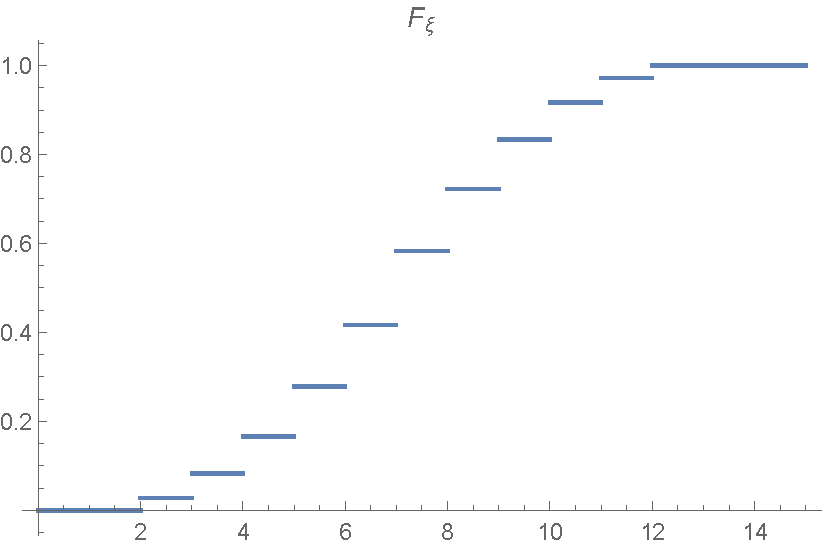
\includegraphics[scale=0.85]{./media/Homework-27-03-20_7.pdf}}
\end{figure}

\subsection*{Задача 5.}
Монета подбрасывается 5 раз,
\begin{enumerate}
	\item[а)] $\xi$ - число орлов, $F_{\xi} - ?$;
	\item[б)] $\xi_1$ - "число орлов"\, - "число решек"\, $F_{\xi_1} - ?$
\end{enumerate}

\noindent \textit{Решение:}

Формула Бернулли:
\[ P_n^k = C_n^k p^k q^{n-k} \]
\noindent где $p$ - вероятность наступления события $A$ (в нашем случае - выпадение орла), которое наступило $k$ раз в $n$ независимых испытаниях, $q=1-p$.

\begin{enumerate}
	\item[а)] Вероятность выпадения как аверса, так и реверса равны $p = \frac{1}{2}$. 
	
		Таким образом, формула для вычислений:
		\[ P(\xi = k) = C_5^k p^k (1 - p)^{n-k} = C_5^k \cdot \left(\frac{1}{2}\right)^k \cdot \left(\frac{1}{2}\right)^{5-k} \]
		\[ P(\xi = 0) = P(\xi = 5) = \underset{=1}{C_5^5} \cdot 
		\begin{cases}
			\left(\frac{1}{2}\right)^1 \cdot \left(\frac{1}{2}\right)^4 = \frac{1}{32} \\
			\left(\frac{1}{2}\right)^5 \cdot \left(\frac{1}{2}\right)^0 = \frac{1}{32}
		\end{cases}
		= \frac{1}{32}
		\]
		\[ P(\xi = 1) = P(\xi = 4) = \frac{5}{32} \]
		\[ P(\xi = 2) = P(\xi = 3) = \frac{10}{32} \]
		
		Следовательно, функция распределения случайной величины выпадения орлов равна:
		\[
		F_{\xi}(x) = \sum_{i=0}^{k<x} P(\xi = k) =
		\begin{cases}
			\frac{1}{32}, &x \in (0,1] \\
			\frac{6}{32} = \frac{3}{16}, &x \in (1,2] \\
			\frac{16}{32} = \frac{1}{2}, &x \in (2,3] \\
			\frac{26}{32} = \frac{13}{16}, &x \in (3,4] \\
			\frac{31}{32}, &x \in (4,5] \\
			1, &x > 5
		\end{cases}
		\]
		График данной функции:
		\begin{figure}[H]
			\center{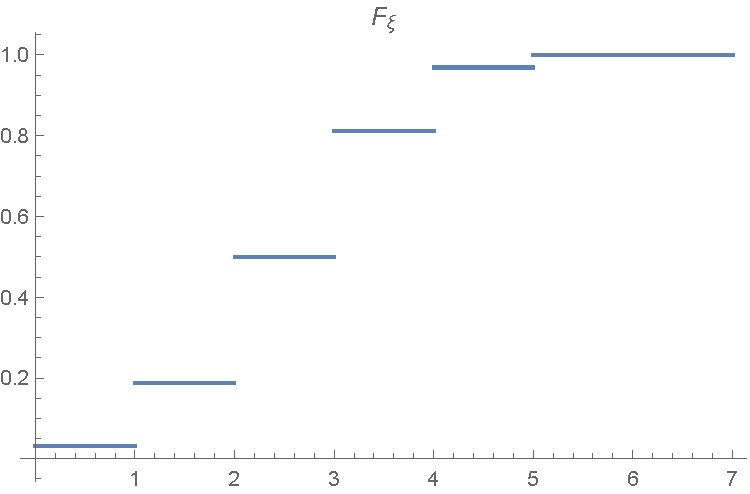
\includegraphics[scale=0.85]{./media/Homework-27-03-20_8.pdf}}
		\end{figure}

	\item[б)] Случайная величина $\xi_1$ однозначно определяется $\xi$, т.к. при условии, что не выпадет орёл, обязательно выпадет решка. Т.е. $\xi_1 = \xi - (5 - \xi) = 2\xi - 5$.
	
	Значит, функция распределения обозначенной случайной величины будет равна:
	\[
	F_{\xi_1}(x) = 
	\begin{cases}
		0, &x \le -5 \\
		\frac{1}{32}, &x \in (-5,-3] \\
		\frac{6}{32} = \frac{3}{16}, &x \in (-3,-1] \\
		\frac{16}{32} = \frac{1}{2}, &x \in (-1,1] \\
		\frac{26}{32} = \frac{13}{16}, &x \in (1,3] \\
		\frac{31}{32}, &x \in (3,5] \\
		1, &x > 5
	\end{cases}
	\]
	График данной функции:
	\begin{figure}[H]
		\center{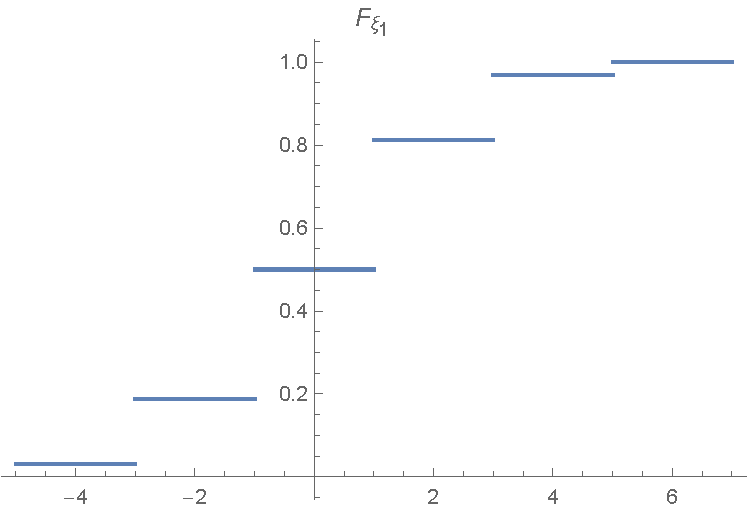
\includegraphics[scale=0.85]{./media/Homework-27-03-20_9.pdf}}
	\end{figure}
	
	Совмещая данные графики, получаем подтверждение утверждения выдвинутого в б) пункте: $\xi_1 = 2\xi - 5$.
	\begin{figure}[H]
		\center{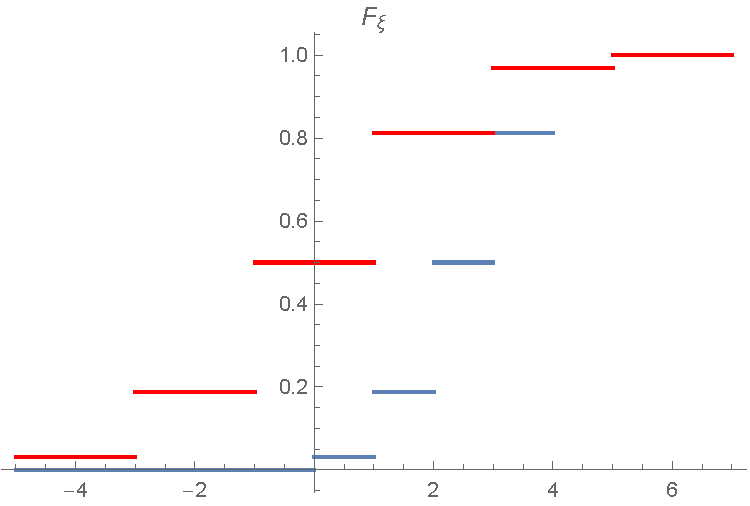
\includegraphics[scale=0.85]{./media/Homework-27-03-20_10.pdf}}
	\end{figure}
\end{enumerate}

\subsection*{Задача 6.}

Точка бросается наугад в $[0,1] \times [0,1]$ - квадрат на плоскости. $\xi$ - сумма координат точки. $F_{\xi} - ?$

\noindent \textit{Решение:}

Переформулируем данную задачу так, чтобы рассматривать отдельно каждую координату точки на интервале $[0,1]$, аналогично 3-ей задачи. В данном случае через квадрат проходит множество прямых, удовлетворяющих уравнение $y=kx+c$ (рассматриваем их отрезки, лежащие внутри площади), при фиксированном $k=1$ и $c \in [0,2]$. Т.е. какую бы точку мы не бросили на плоскость квадрата, она всё равно будет лежать на одной их таких прямых, при том все остальные точки, лежащие на этой прямой, будут иметь равную сумму координат.
\begin{figure}[H]
	\center{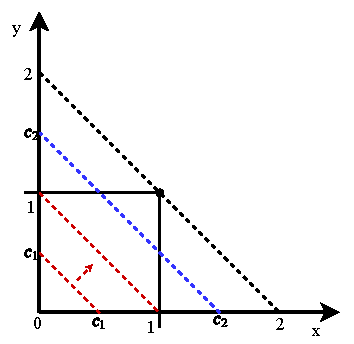
\includegraphics[scale=1]{./media/Homework-27-03-20_11.pdf}}
\end{figure}
Примем $\xi = c$ (в общем случаем сумма координат точки на прямой будет равняться $2 \cdot c$, но данный коэффициент в данном случае роли не играет). Тогда $\xi < x$ при $x \in (0,1]$ (на рис. обозначено красным) случайная величина будет равняться площади прямоугольного $\triangle$-ка с катетами равными $x = y$. Для $\xi < x$ при $x \in (1,x]$ (на рис. обозначено синим) случайная величина будет равняться разности площади квадрата и прямоугольного $\triangle$-ка (на рис. ниже обозначен зелёным) с катетами равными $2-x = 2-y$ (2 - предельная точка, при которой отрезок прямой лежит внутри площади квадрата).
\begin{figure}[H]
	\center{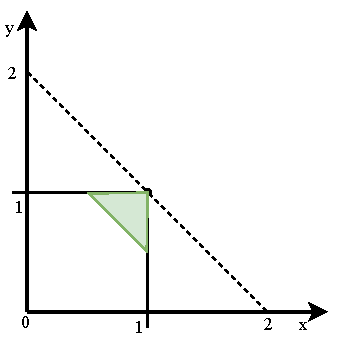
\includegraphics[scale=1]{./media/Homework-27-03-20_12.pdf}}
\end{figure}
В результате, площадь квадрата равна $1^2=1$, площадь прямоугольного $\triangle$-ка с катетами по $x$ равна $\frac{1}{2}x^2$.

Функция распределения случайной величины $\xi$ примет вид:
\[
F_{\xi} (x) =
\begin{cases}
	0, &x \le 0 \\
	\frac{x^2}{2}, &x \in (0,1] \\
	1 - \frac{(2-x)^2}{2}, &x \in (1,2] \\
	1, &x>2
\end{cases}
\]
График полученной функции представлен ниже:
\begin{figure}[H]
	\center{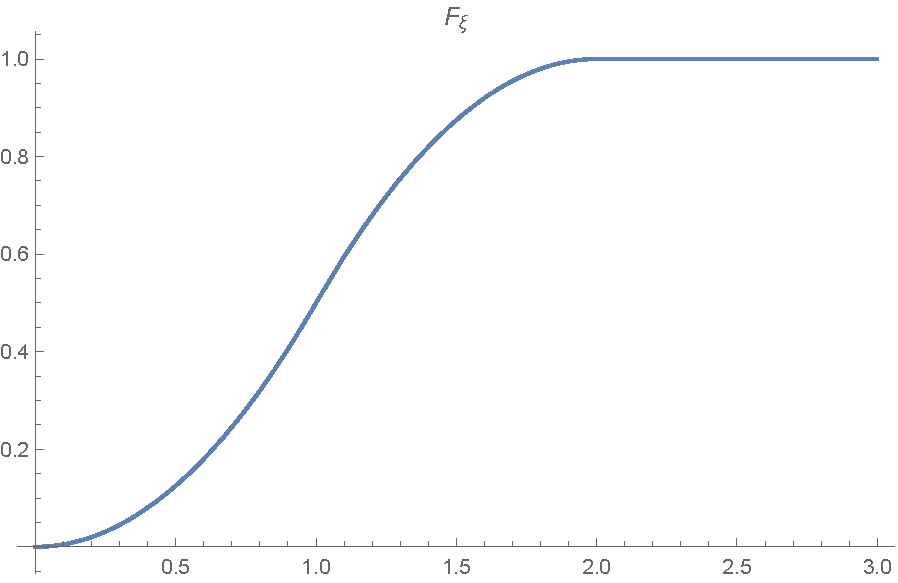
\includegraphics[scale=0.85]{./media/Homework-27-03-20_13.pdf}}
\end{figure}

\section*{Дискретные и абсолютно непрерывные случайные величины}

\noindent Распределение $\xi$ - дискретное, если $\exists E$ - не более чем счётное, т.е. $P(\xi \in E) = 1$.

\noindent Распределение $\xi$ - абсолютно непрерывное, если $\exists p_{\xi}$ - неотрицательная измеримая, т.ч. 

\noindent $F_{\xi} = \int\limits_{-\infty}^{x} p_{\xi} (t)dt, \forall t \in \mathbb{R}$ ($p_{\xi}$ - плотность распределения).

\noindent В рассмотренных ранее задачах:
\begin{enumerate}
	\item $\xi$ - дискретная, $E = \{1,2,\dots,6\}$
	\item $\xi$ - дискретная, $E = \mathbb{N} \cup \{0\}$
	\item $\xi$ - абсолютно непрерывная,
	\[ p_{\xi} =
	\begin{cases}
		1, x \in [0,1] \\
		0, x \notin [0,1]
	\end{cases}
	\]
\end{enumerate}

Абсолютно-непрерывные величины, связь плотности и функции распределения:
\[ F_{\xi} = \int_{-\infty}^{x} p_{\xi} (t) dt \]
\[ p_{\xi}(t) = F_{\xi}'(x) \]
в точках, где производная $\exists$-ет.

\subsection*{Задача 7.}

Светофор работает циклически:
\begin{figure}[H]
	\center{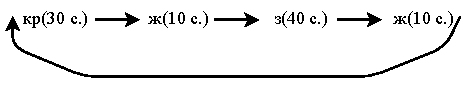
\includegraphics[scale=1.15]{./media/Homework-27-03-20_14.pdf}}
\end{figure}
$\xi$ - время ожидания 'з' сигнала светофора а/м, который подъезжает к светофору в случайный момент времени.

\noindent \textit{Решение:}

\noindent $\omega$ - точка на окружности (приезд а/м). $\xi(\omega)$ - длина дуги от $\omega$ до начала 'з'.

\noindent Геометрическая схема: $P(\omega \in A) = \dfrac{\text{Длина дуги } A}{\text{Длина окружности}}$
\begin{figure}[H]
	\center{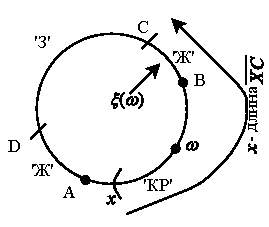
\includegraphics[scale=1.2]{./media/Homework-27-03-20_15.pdf}}
\end{figure}
\[ P(\xi < 0) = 0 \]
\[ P(\xi = 0) = \frac{\text{Длина дуги 'з'}}{\text{Длина окр.}} = \frac{40}{30 + 10 + 40 + 10} = \frac{4}{9} \]
\[ P(\xi < x) = \frac{\text{Длина дуги } \overline{XC}}{\text{Длина окр.}} = \frac{x+40}{90} = \frac{4}{9} + \frac{x}{90}, x \in (0,50) \]
\[ P(\xi < x) = 1, x < 50 \]
\begin{remark}
	Не дискретное и не абсолютно непрерывная - СМЕСЬ.
\end{remark}
\[ F_{\xi} (x) = \frac{4}{9} F_d (x) + \frac{5}{9} F_c(x) \]
\[
F_d(x) =
\begin{cases}
	0, x \le 0 \\
	1, x > 0
\end{cases}
F_c =
\begin{cases}
	0, x \le 0 \\
	\frac{x}{50}, x \in (0,50] \\
	1, x > 50
\end{cases}
\]
\begin{figure}[H]
	\center{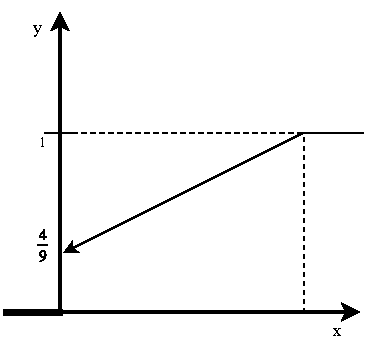
\includegraphics[scale=1]{./media/Homework-27-03-20_16.pdf}}
\end{figure}

\subsection*{Задача 8.}

$\xi$ - дискретная, $P(\xi = i)$ задана таблицей распределения. $F\xi(x) - ?$
\begin{table}[H]
	\centering\makegapedcells
	\begin{tabular}{|c|c|c|c|c|c|c|}
		\hline
		$i$  & 0             & 1             & 2             & 3              & 4              & $\Sigma$ \\ \hline
		вер. & $\frac{1}{8}$ & $\frac{1}{4}$ & $\frac{1}{2}$ & $\frac{1}{16}$ & $\frac{1}{16}$ & 1        \\ \hline
	\end{tabular}
\end{table}

\noindent \textit{Решение:}

\[ F_{\xi} = \sum_{i=0}^{i<x} P(\xi = i) =
\begin{cases}
	0, &x \le 0 \\
	\frac{1}{8}, &x \in (0,1] \\
	\frac{1}{8} + \frac{1}{4} = \frac{3}{8}, &x \in (1,2] \\
	\frac{1}{8} + \frac{1}{4} + \frac{1}{2} = \frac{7}{8}, &x \in (2,3] \\
	\frac{1}{8} + \frac{1}{4} + \frac{1}{2} + \frac{1}{16} = \frac{15}{16}, &x \in (3,4] \\
	1, &x > 4
\end{cases}
\]
График распределения данной дискретной случайной величины:
\begin{figure}[H]
	\center{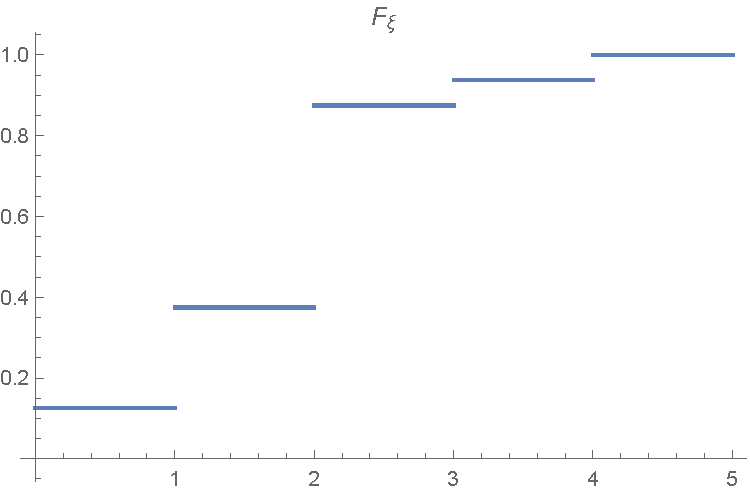
\includegraphics[scale=0.8]{./media/Homework-27-03-20_17.pdf}}
\end{figure}

\subsection*{Задача 9.}

$\xi$ - дискретная,  $F_{\xi}(x)$ задана таблицей. Построить таблицу распределения.
\begin{table}[H]
	\centering\makegapedcells
	\begin{tabular}{|c|c|c|c|c|c|}
		\hline
		$x$          & $\le -1$ & $(-1,0]$      & $(0,\frac{1}{2}]$ & $(\frac{1}{2},1]$ & $(1,\infty]$ \\ \hline
		$F_{\xi}(x)$ & $0$      & $\frac{1}{4}$ & $\frac{1}{2}$     & $\frac{3}{4}$     & $1$          \\ \hline
	\end{tabular}
\end{table}

\noindent \textit{Решение:}

Строим график данной функции:
\begin{figure}[H]
	\center{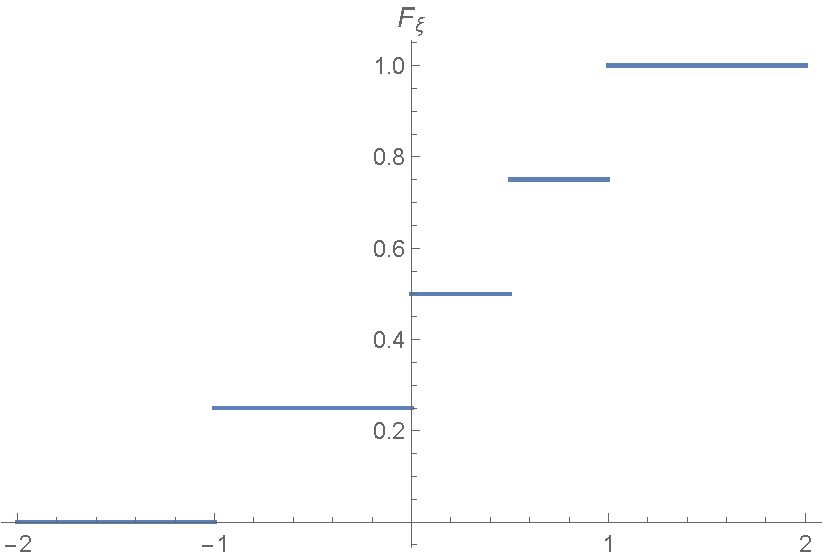
\includegraphics[scale=0.8]{./media/Homework-27-03-20_18.pdf}}
\end{figure}
Строим таблицу распределения:
\begin{table}[H]
	\centering\makegapedcells
	\begin{tabular}{|c|c|c|c|c|}
		\hline
		$i$          & $-1$         & $0$                                       & $\frac{1}{2}$                             & $1$                             \\ \hline
		$P(\xi = i)$ & $\frac{1}{4}$ & $\frac{1}{2} - \frac{1}{4} = \frac{1}{4}$ & $\frac{3}{4} - \frac{1}{2} = \frac{1}{4}$ & $1 - \frac{3}{4} = \frac{1}{4}$ \\ \hline
	\end{tabular}
\end{table}
Проверяем, например, для $x \in (0,\frac{1}{2}]: \frac{1}{4} + \frac{1}{4} = \frac{1}{2}$ - всё верно.

\subsection*{Задача 10.}

В Задаче №4 определить тип случайной величины $\xi$. Характеризовать распределение с помощью таблицы распределения или плотности распределения.

\noindent \textit{Решение:}

Т.к. $\exists E$ не более, чем счётное, т.е. $E = \{ 2,3,\dots,12 \} \Rightarrow$ величина $\xi$ - \underline{дискретная}.

Таблица распределения:
\begin{table}[H]
	\centering\makegapedcells
	\begin{tabular}{|c|c|c|c|c|c|c|c|c|c|c|c|}
		\hline
		$i$          & 2              & 3                                                     & 4                                                     & 5                                        & 6              & 7                          & 8              & 9             & 10             & 11             & 12             \\ \hline
		$P(\xi = i)$ & $\frac{1}{36}$ & $\frac{1}{12}-\frac{1}{36}=\frac{2}{36}=\frac{1}{18}$ & $\frac{6}{36}-\frac{3}{36}=\frac{3}{36}=\frac{1}{12}$ & $\frac{10}{36}-\frac{6}{36}=\frac{1}{9}$ & $\frac{5}{36}$ & $\frac{6}{36}=\frac{1}{6}$ & $\frac{5}{36}$ & $\frac{1}{9}$ & $\frac{1}{12}$ & $\frac{1}{18}$ & $\frac{1}{36}$ \\ \hline
	\end{tabular}
\end{table}

\subsection*{Задача 11.}

Дана плотность абсолютно непрерывного распределения $\xi$
\[
p_{\xi} =
\begin{cases}
	e^{-x}, x \ge 0 \\
	0, x < 0
\end{cases}
\]

Найти $F_{\xi}(x) - ?$

\noindent \textit{Решение:}

\[ F_{\xi} (x) =
\begin{cases}
	0, x \le 0 \\
	\int_{0}^{x} e^{-t} dt = 1 - e^{-x}, x>0
\end{cases}
\]
\begin{figure}[H]
	\center{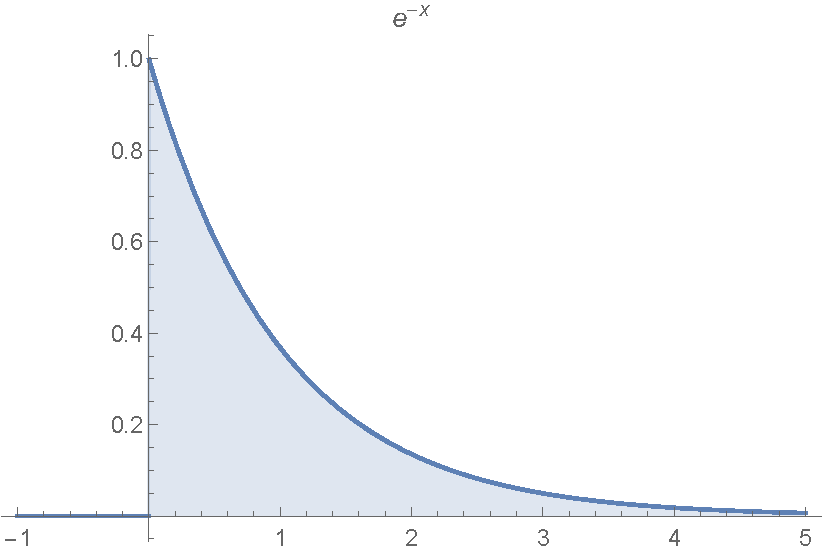
\includegraphics[scale=0.75]{./media/Homework-27-03-20_19.pdf}}
\end{figure}

\subsection*{Задача 12.}

Дана $F_{\xi}$
\[ F_{\xi} =
\begin{cases}
	0, x \le 0 \\
	x^2, x \in (0,1] \\
	1, x > 1
\end{cases}
\]
Найти $p_{\xi}(x) - ?$

\noindent \textit{Решение:}

\[
F_{\xi}' =
\begin{cases}
	2x, x \in (0,1) \\
	0, x \notin [0,1]
\end{cases} -
\text{ не дифф. в } \{0,1\}
\]
\[
p_{\xi} =
\begin{cases}
	2x, x \in (0,1) \\
	0, x \notin [0,1]
\end{cases}
\]
Проверка:
\[
\int_{-\infty}^{\infty} p_{\xi} dx = \int_{0}^{1} 2x dx = 1
\]
$p_{\xi}$ - плотность распределения.

\subsection*{Задача 13.}

Плотность распределения:
\[
p_{\xi}(x) =
\begin{cases}
	e^{2x} \cdot c, x \le 0 \\
	0, x > 0
\end{cases}
\]
Найти $c - ?$

\noindent \textit{Решение:}

\[ 1 = \int_{-\infty}^{\infty} p_{\xi} (x) dx = \int_{-\infty}^{0} c \cdot e^{2x} = \frac{ce^{2x}}{2} \bigg|_{-\infty}^0 \]
\[ \Rightarrow \frac{c}{2} = 1 \Rightarrow c = 2 \]

\subsection*{Задача 14.}

\[
F_{\xi}(x) =
\begin{cases}
	0, x \le 0 \\
	\sin(x), x \in \left(0, \frac{\pi}{2}\right] \\
	1, x > \frac{\pi}{2}
\end{cases}
\]
Найти $p_{\xi} - ?$

\noindent \textit{Решение:}

Построим график данной функции:
\begin{figure}[H]
	\center{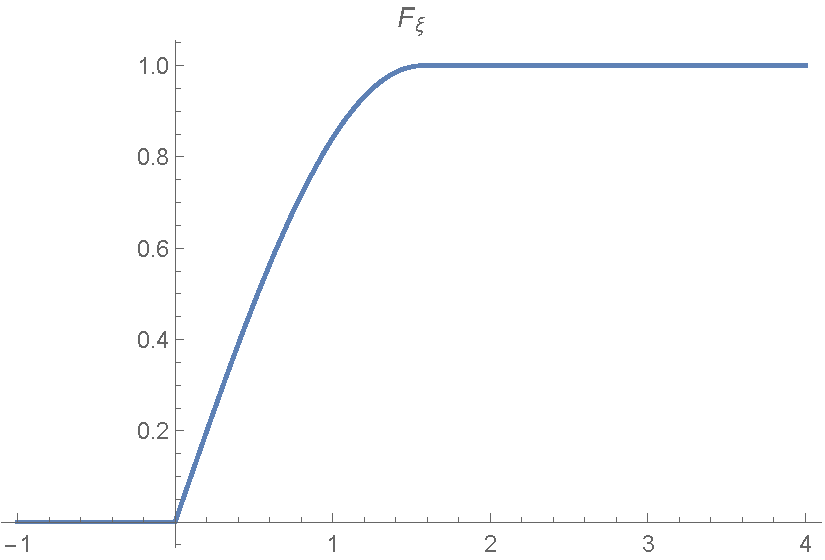
\includegraphics[scale=0.8]{./media/Homework-27-03-20_20.pdf}}
\end{figure}
\[
F_{\xi}'(x) =
\begin{cases}
	\cos(x), x \in \left(0, \frac{\pi}{2}\right) \\
	0, x \notin \left[0, \frac{\pi}{2}\right]
\end{cases}
\]
Как видно и аналитически, и графически, функция не дифференцируема в точках 0 и $\frac{\pi}{2}$.
\[ p_{\xi}(t) = F_{\xi}'(x) \Rightarrow \]
\[
p_{\xi}(x) =
\begin{cases}
	\cos(x), x \in \left(0, \frac{\pi}{2}\right) \\
	0, x \notin \left[0, \frac{\pi}{2}\right]
\end{cases}
\]

\subsection*{Задача 15.}

\[
p_{\xi} =
\begin{cases}
	0, x \le -1 \text{ или } x > 1 \\
	\frac{1}{3}, x \in (-1,0] \\
	c, x \in (0,1]
\end{cases}
\]
Найти $c - ?, F_{\xi} - ?$

\noindent \textit{Решение:}
\[ F_{\xi} = \int_{-\infty}^{x} p_{\xi} (t) dt \]
\[ p_{\xi}(t) = F_{\xi}'(x) \]

\[ 1 = \int_{-\infty}^{\infty} p_{\xi} (x) = \int_{-1}^{0} \frac{1}{3}dx + \int_{0}^{1} c dx = \frac{1}{3} + c \]
\[ \Rightarrow c = \frac{2}{3} \]
Построим график полученной функции:
\begin{figure}[H]
	\center{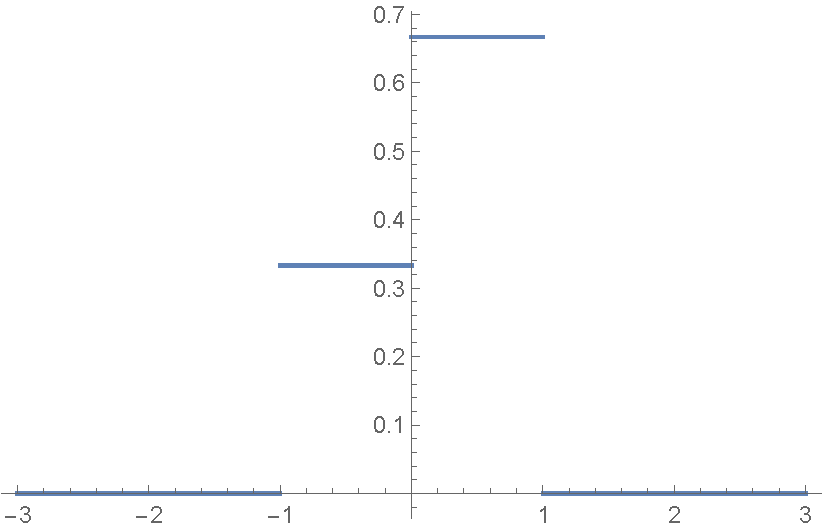
\includegraphics[scale=0.8]{./media/Homework-27-03-20_21.pdf}}
\end{figure}

\begin{itemize}
	\item $\int\limits_{-\infty}^{x}0dt = 0$
	\item $\int\limits_{-1}^{x} \frac{1}{3}dt = \frac{1}{3}x + \frac{1}{3}$
	\item $\int\limits_{-1}^{0} \frac{1}{3} dt + \int\limits_{0}^x \frac{2}{3}dt = \frac{2}{3}x + \frac{1}{3}$
\end{itemize}
\[ \Rightarrow F_{\xi}(x) = 
\begin{cases}
	0, &x \le -1 \\
	\frac{1}{3}x + \frac{1}{3}, &x \in (-1,0] \\
	\frac{2}{3}x + \frac{1}{3}, &x \in (0,1] \\
	1, &x > 1
\end{cases}
\]
Построим график полученной функции:
\begin{figure}[H]
	\center{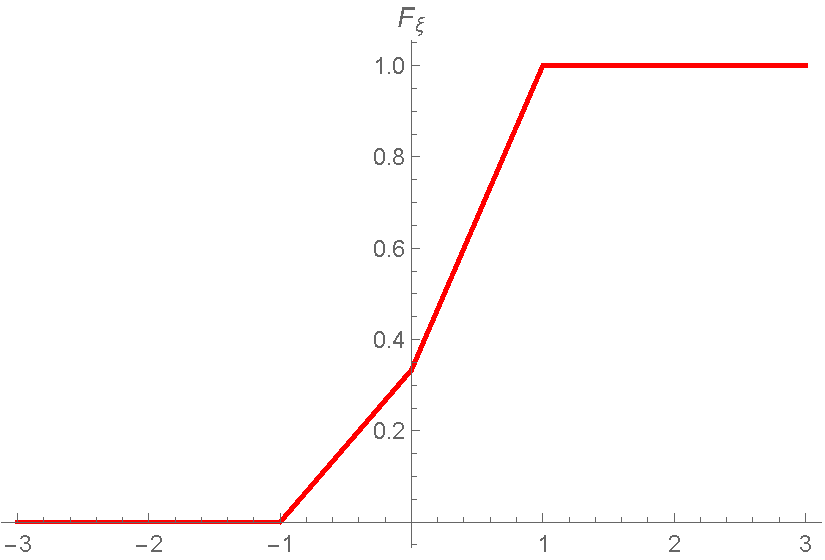
\includegraphics[scale=0.8]{./media/Homework-27-03-20_22.pdf}}
\end{figure}

\subsection*{Задача 16.}

\[
p_{\xi}(x) =
\begin{cases}
	c \cdot |x|, |x| \le 1 \\
	0, |x| > 1
\end{cases}
\]
Найти $c - ?, F_{\xi}$

\noindent \textit{Решение:}

\noindentПроизводная переменной по модулю равна частному этой переменной к ее модулю.
\[ |x|' = \frac{x}{|x|}, x \ne 0 \]
\noindentИнтеграл переменной по модулю равен:
\[ \int |x|dx = \frac{x \cdot |x|}{2} + C, C \in \mathbb{Z} \]

Раскроем модуль выражений системы и получим:
\[
p_{\xi}(x) =
\begin{cases}
	-cx, -1 \le x \le 0 \\
	cx, 0 \le x \le 1 \\
	0, x < -1 \\
	0, x > 1
\end{cases}
\]
\[ 1 = \int_{-1}^{0} -cx dx + \int_{0}^{1} cx dx = \frac{c}{2} + \frac{c}{2} = c \Rightarrow c = 1 \]
Построим график данной функции и исходной, подставив найденной $с$. Они аналогичны $\to$ вычисления верны.
\begin{figure}[H]
	\center{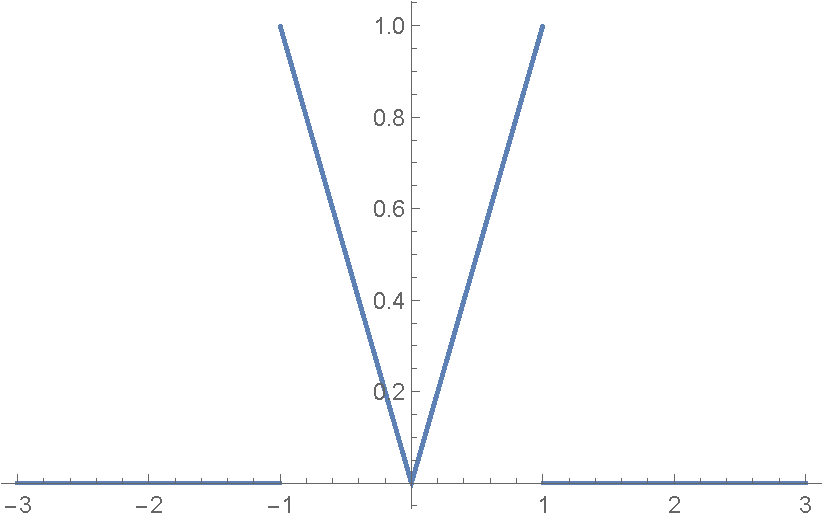
\includegraphics[scale=0.8]{./media/Homework-27-03-20_23.pdf}}
\end{figure}

\[
F_{\xi}(x) =
\begin{cases}
	0, &x \le -1 \\
	\frac{-x^2 + 1}{2}, &-1 < x \le 0 \\
	\frac{x^2}{2} + \frac{1}{2}, &0 < x \le 1 \\
	1, &x > 1
\end{cases}
\]
Построим график полученной функции:
\begin{figure}[H]
	\center{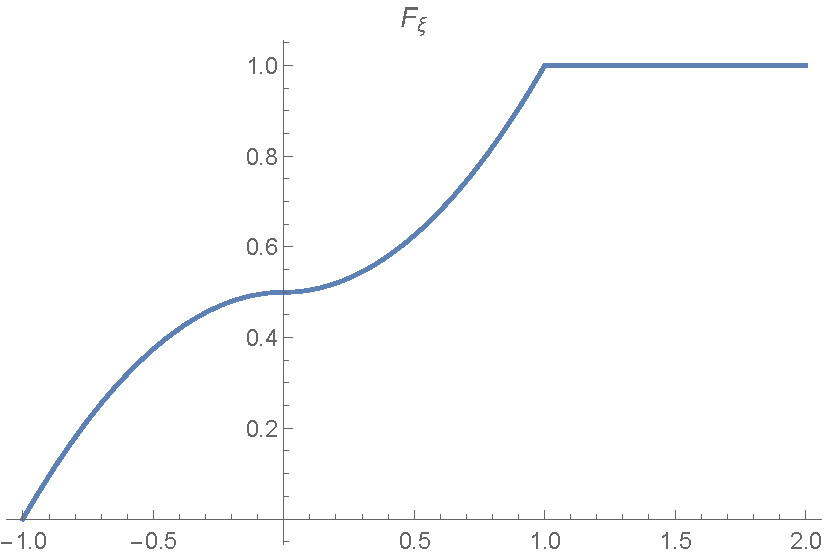
\includegraphics[scale=0.8]{./media/Homework-27-03-20_24.pdf}}
\end{figure}

\subsection*{Задача 17.}

\[ p_{\xi} = c e^{-|x|}, x \in \mathbb{R} \]
Найти $c - ?, F_{\xi} - ?$

\noindent \textit{Решение:}

Раскрываем модуль и получаем:
\[
p_{\xi}(x) =
\begin{cases}
	c \cdot e^x, x < 0 \\
	c \cdot e^{-x}, x \ge 0
\end{cases}
\]
\[
1 = \int_{-\infty}^{0} c \cdot e^x dx + \int_{0}^{\infty} c \cdot e^{-x} dx = c + c \Rightarrow c = \frac{1}{2}
\]
Построим график:
\begin{figure}[H]
	\center{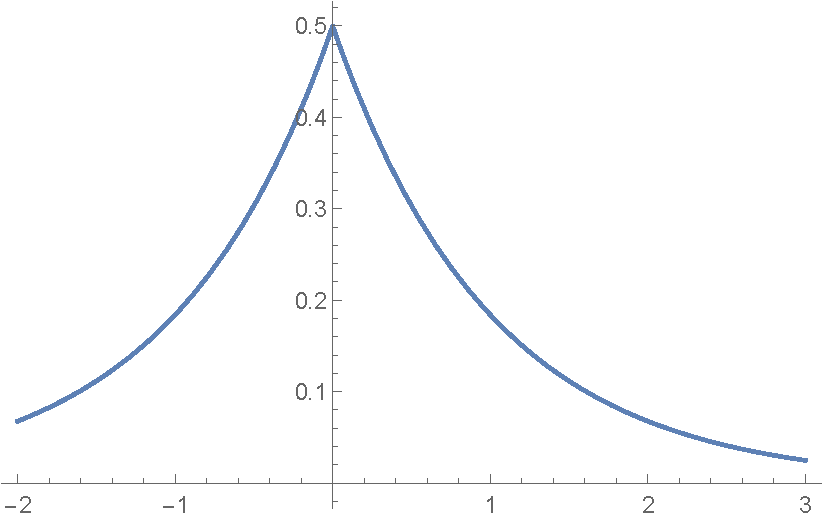
\includegraphics[scale=0.8]{./media/Homework-27-03-20_25.pdf}}
\end{figure}
\begin{itemize}
	\item $\int\limits_{-\infty}^{x} \frac{1}{2} \cdot e^{x} dt = \frac{e^x}{2}$
	\item $\frac{1}{2} + \int\limits_{0}^{x} \frac{1}{2} e^{-x} dt = \frac{1}{2} + \left(-\frac{e^{-x}}{2}\right) \bigg|_{0}^x = \frac{1}{2} + \frac{1}{2} - \frac{e^{-x}}{2} = -\frac{e^{-x}}{2} + 1$
\end{itemize}
\[
\Rightarrow F_{\xi} =
\begin{cases}
	\frac{e^x}{2}, &x \le 0 \\
	-\frac{e^{-x}}{2} + 1, &x > 0
\end{cases}
\]
Построим график:
\begin{figure}[H]
	\center{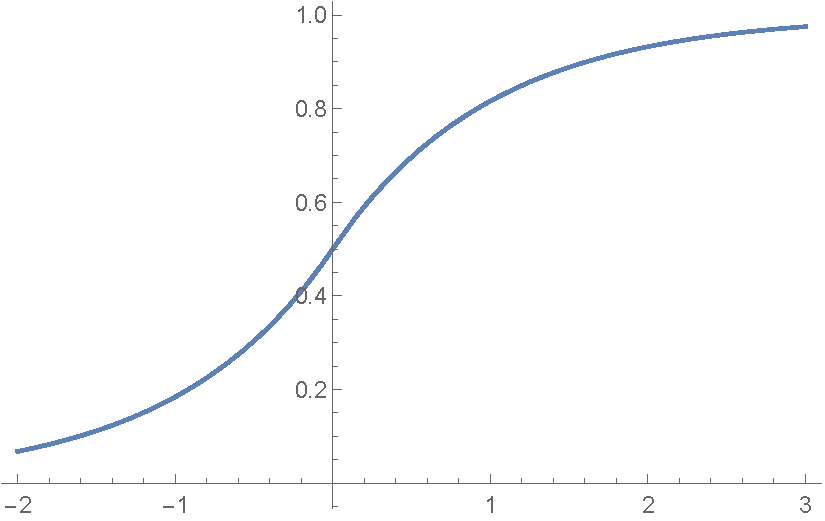
\includegraphics[scale=0.8]{./media/Homework-27-03-20_26.pdf}}
\end{figure}

\end{document} 